I use the definition of decay stated \href{https://en.wikipedia.org/wiki/Particle_decay}{here}. \\
I do not follow the order of the questions as given, but everything is reported here.
\begin{table}[htbp]
    \centering
    \begin{tabular}{cccccc}
        \toprule
            Process & Type & Interaction & Allowed & Suppressed & Reason not allowed \\
        \midrule 
            $1$ & decay & electroweak & yes & no & \\
            $2$ & & & no & & charge \\
            $3$ & decay & electroweak & yes & yes & \\
            $4$ & decay & weak & yes & no & \\
            $5$ & decay & strong & yes & no & \\
            $6$ & reaction & electroweak + strong & yes & no & \\
            $7$ & decay & weak & yes & no & \\
            $8$ & & & no & & lepton number \\
        \bottomrule
    \end{tabular}
\end{table}

\begin{figure}[hbtp]
    \centering
    \begin{minipage}{0.4\textwidth}
        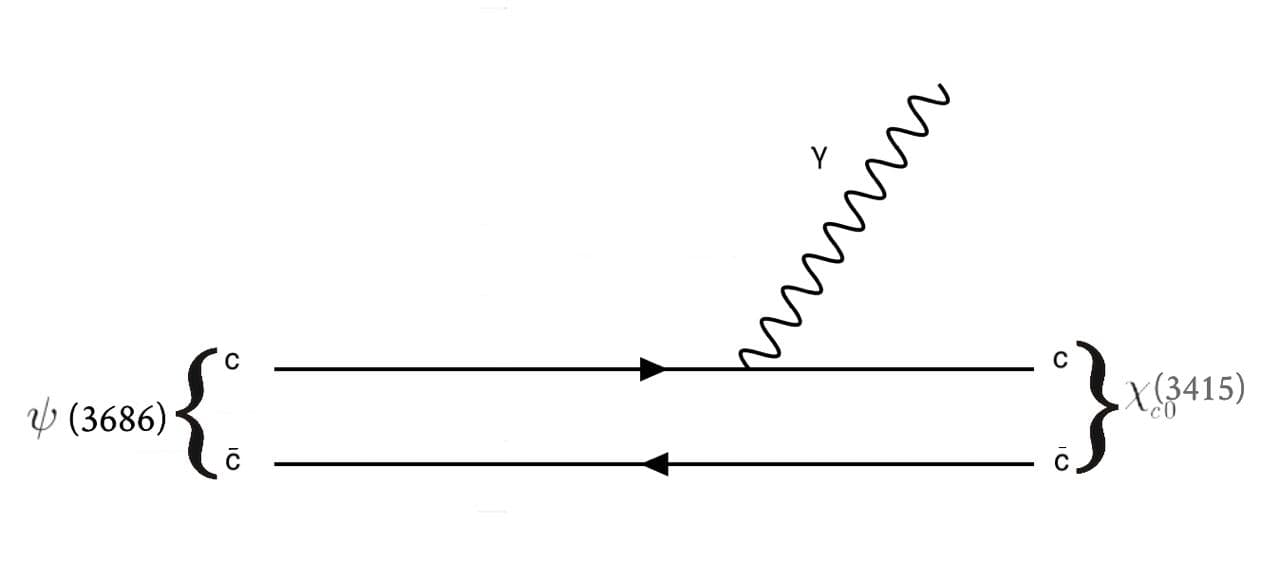
\includegraphics[scale=0.2]{Feynman/feynm1.jpg}
        \caption{$\psi(3686) \to \chi_{0}(3145) + \gamma$}
    \end{minipage}
    \hspace{0.1\textwidth}
    \begin{minipage}{0.4\textwidth}
        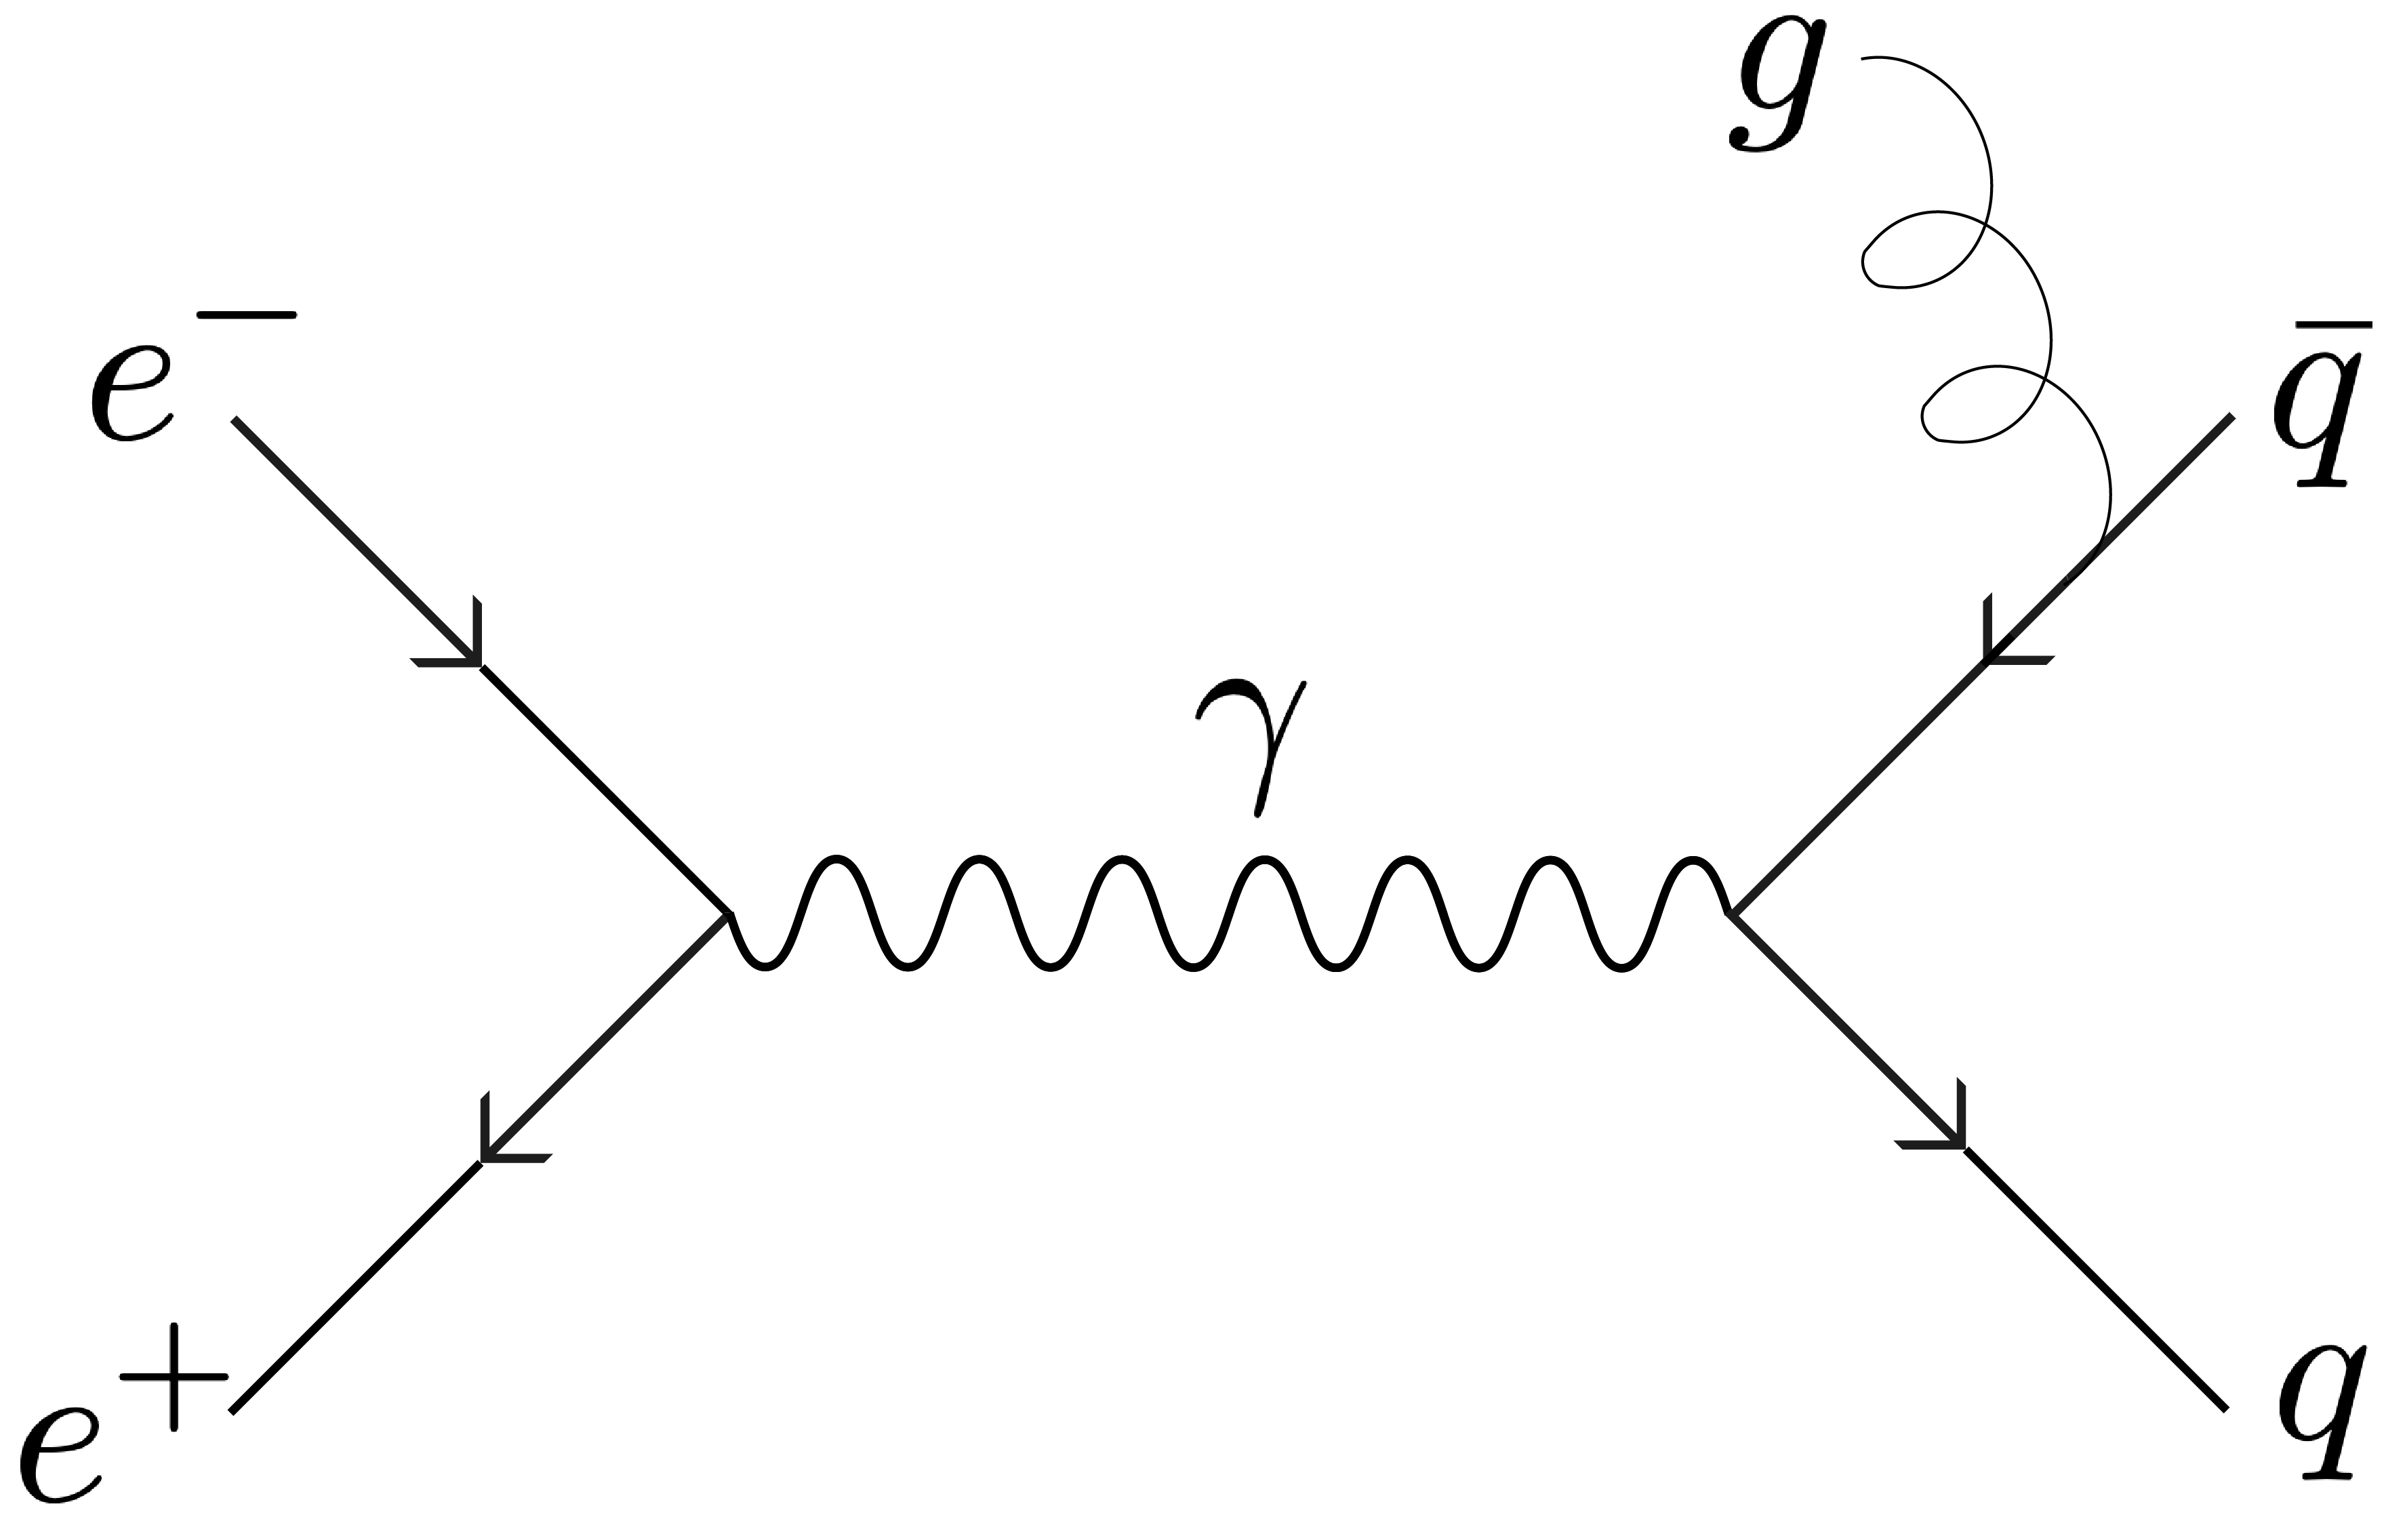
\includegraphics[scale=0.25]{Feynman/eeqq-01.jpg}
        \caption{$b \to s \gamma$}
    \end{minipage}
    \vspace{30pt}
    \begin{minipage}{0.4\textwidth}
        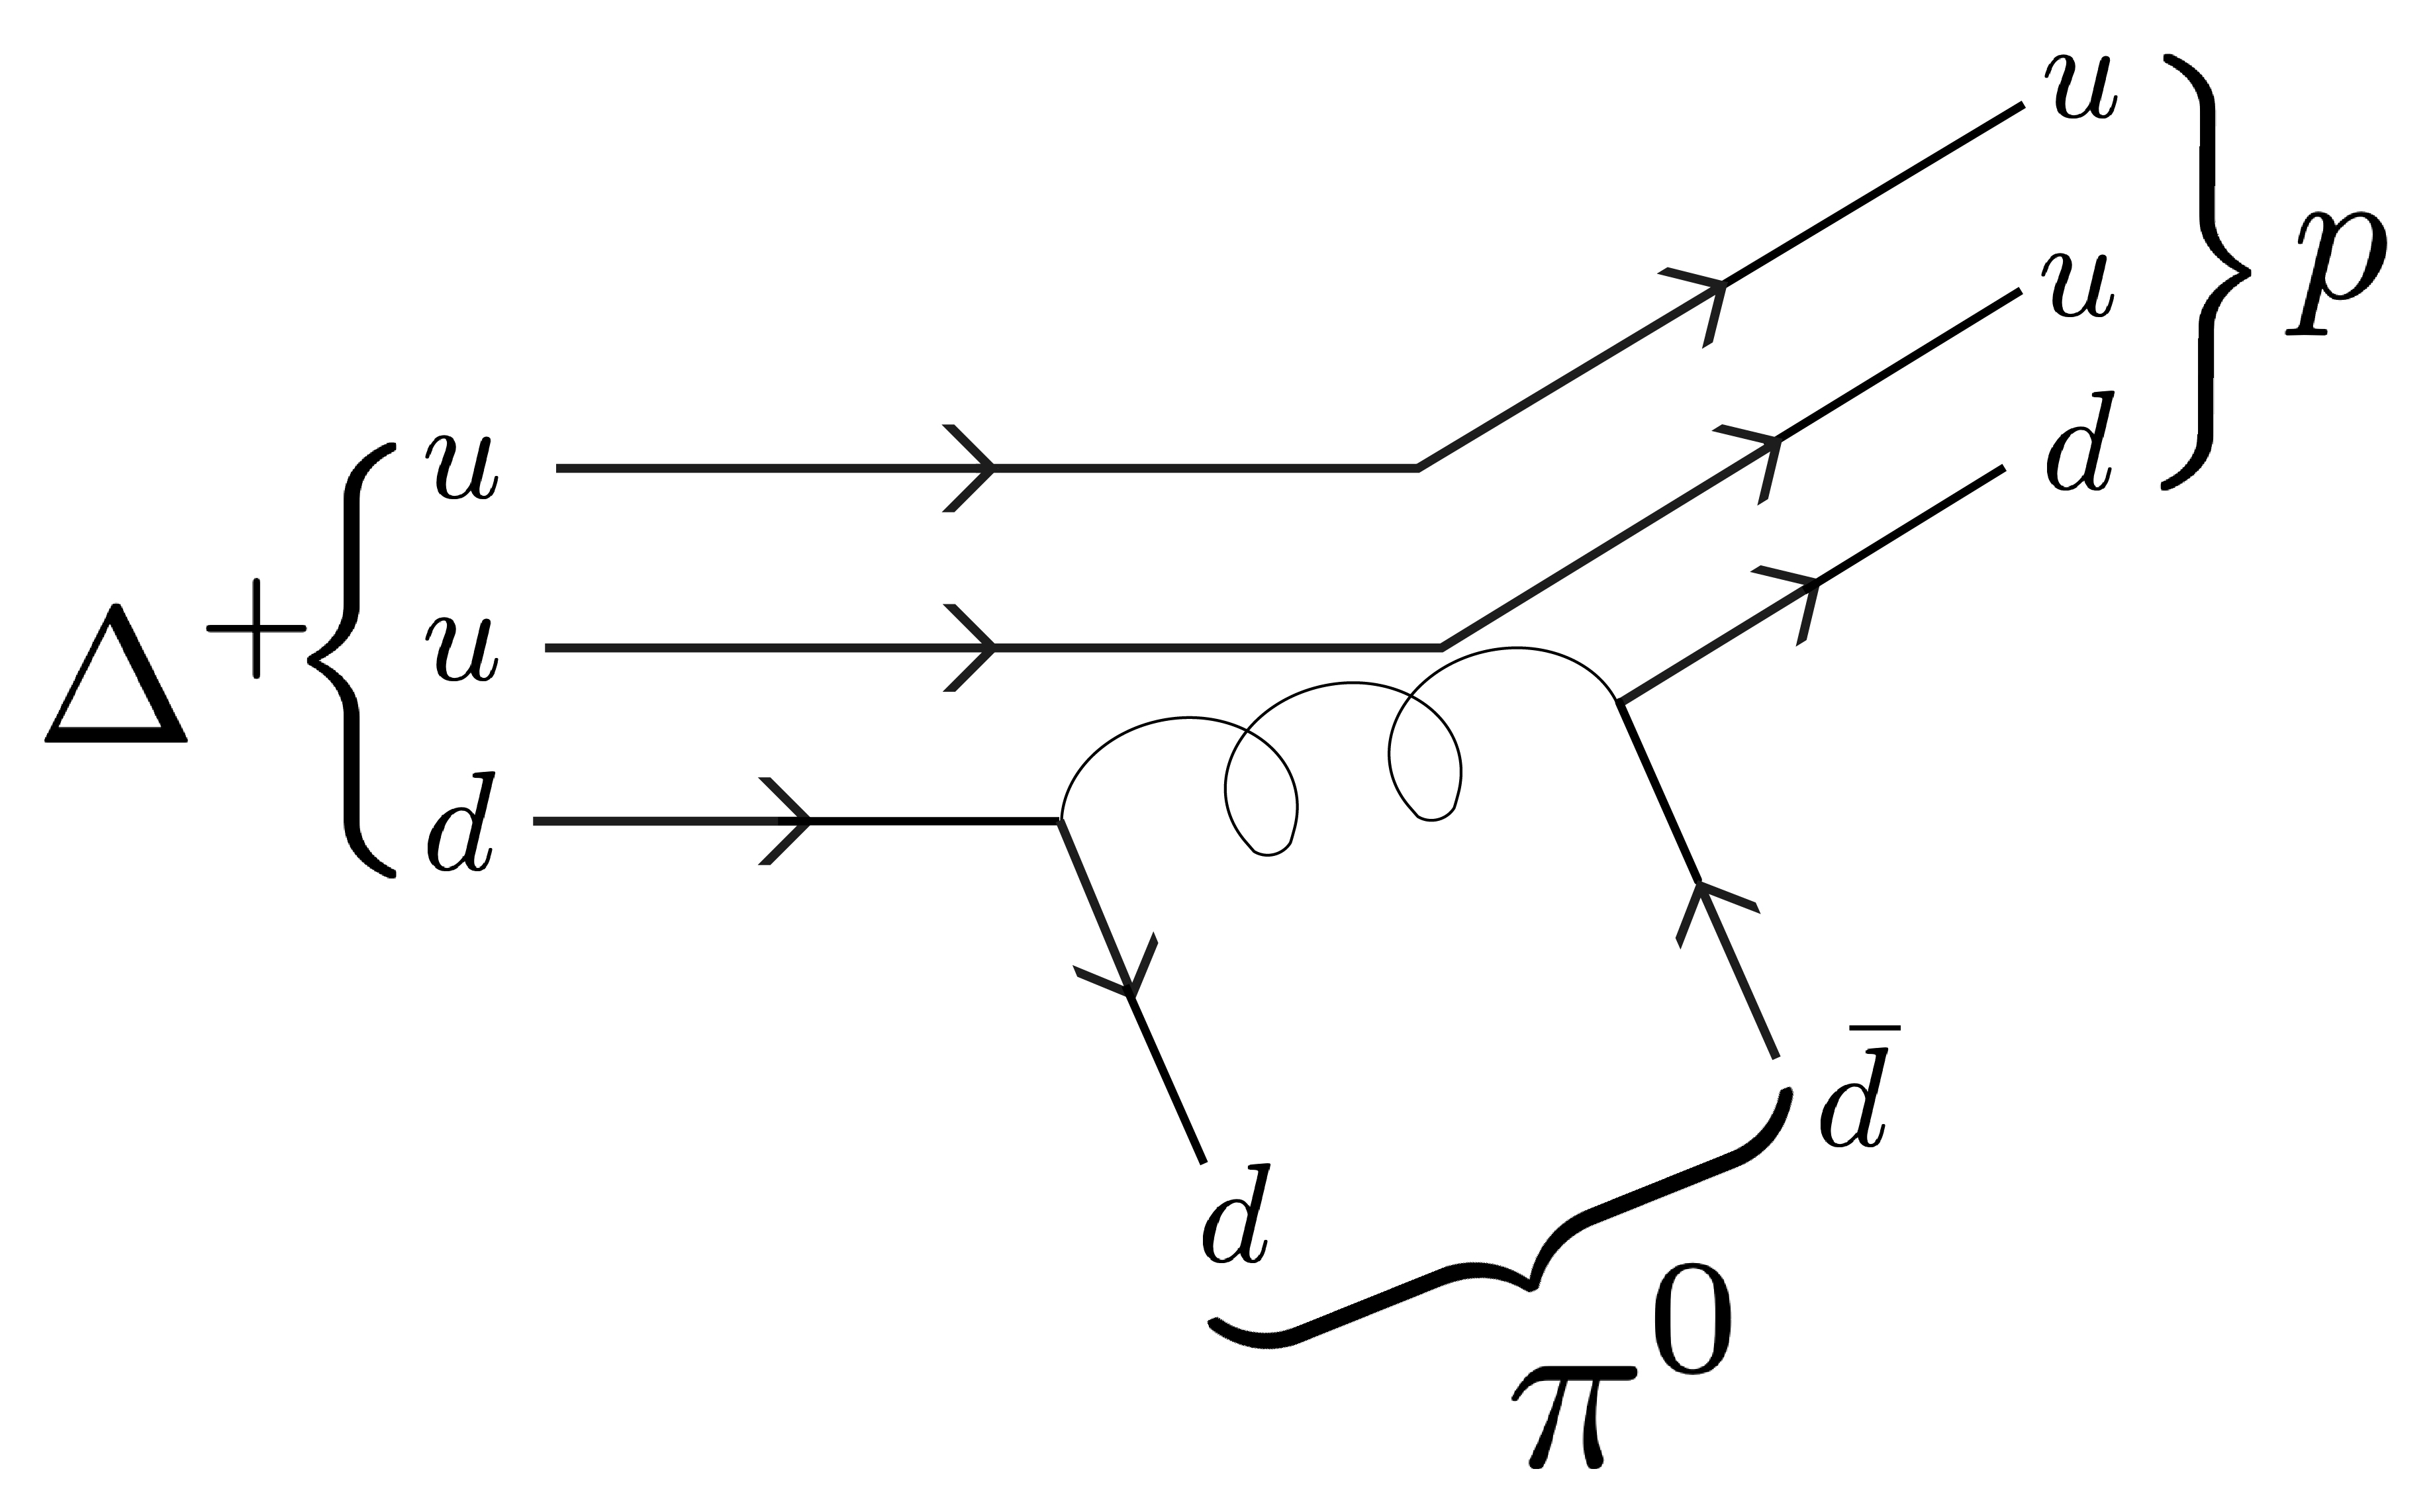
\includegraphics[scale=0.045]{Feynman/Delta+-01.jpg}
        \caption{$ \Delta^+ \to p \pi^0$}
    \end{minipage}
    \hspace{0.1\textwidth}
    \begin{minipage}{0.4\textwidth}
        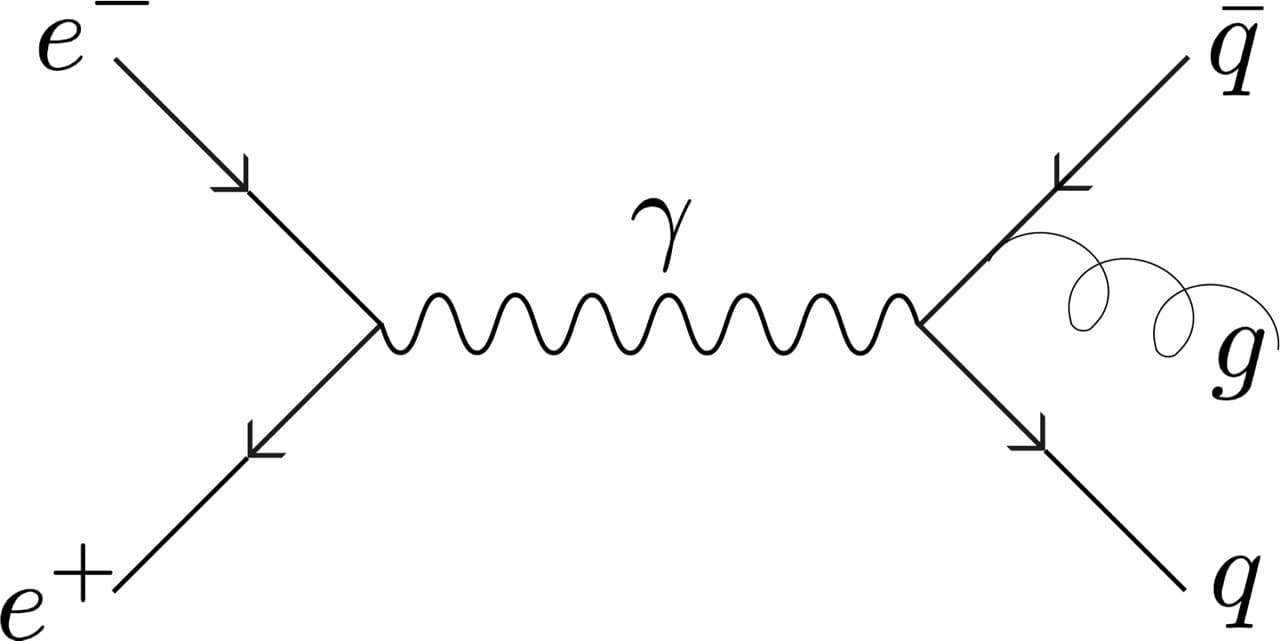
\includegraphics[scale=0.3]{Feynman/decaycircular.jpg}
        \caption{$e^+ e^- \to q \Bar{q} g$}
    \end{minipage}
    \vspace{30pt}
    \begin{minipage}{0.4\textwidth}
        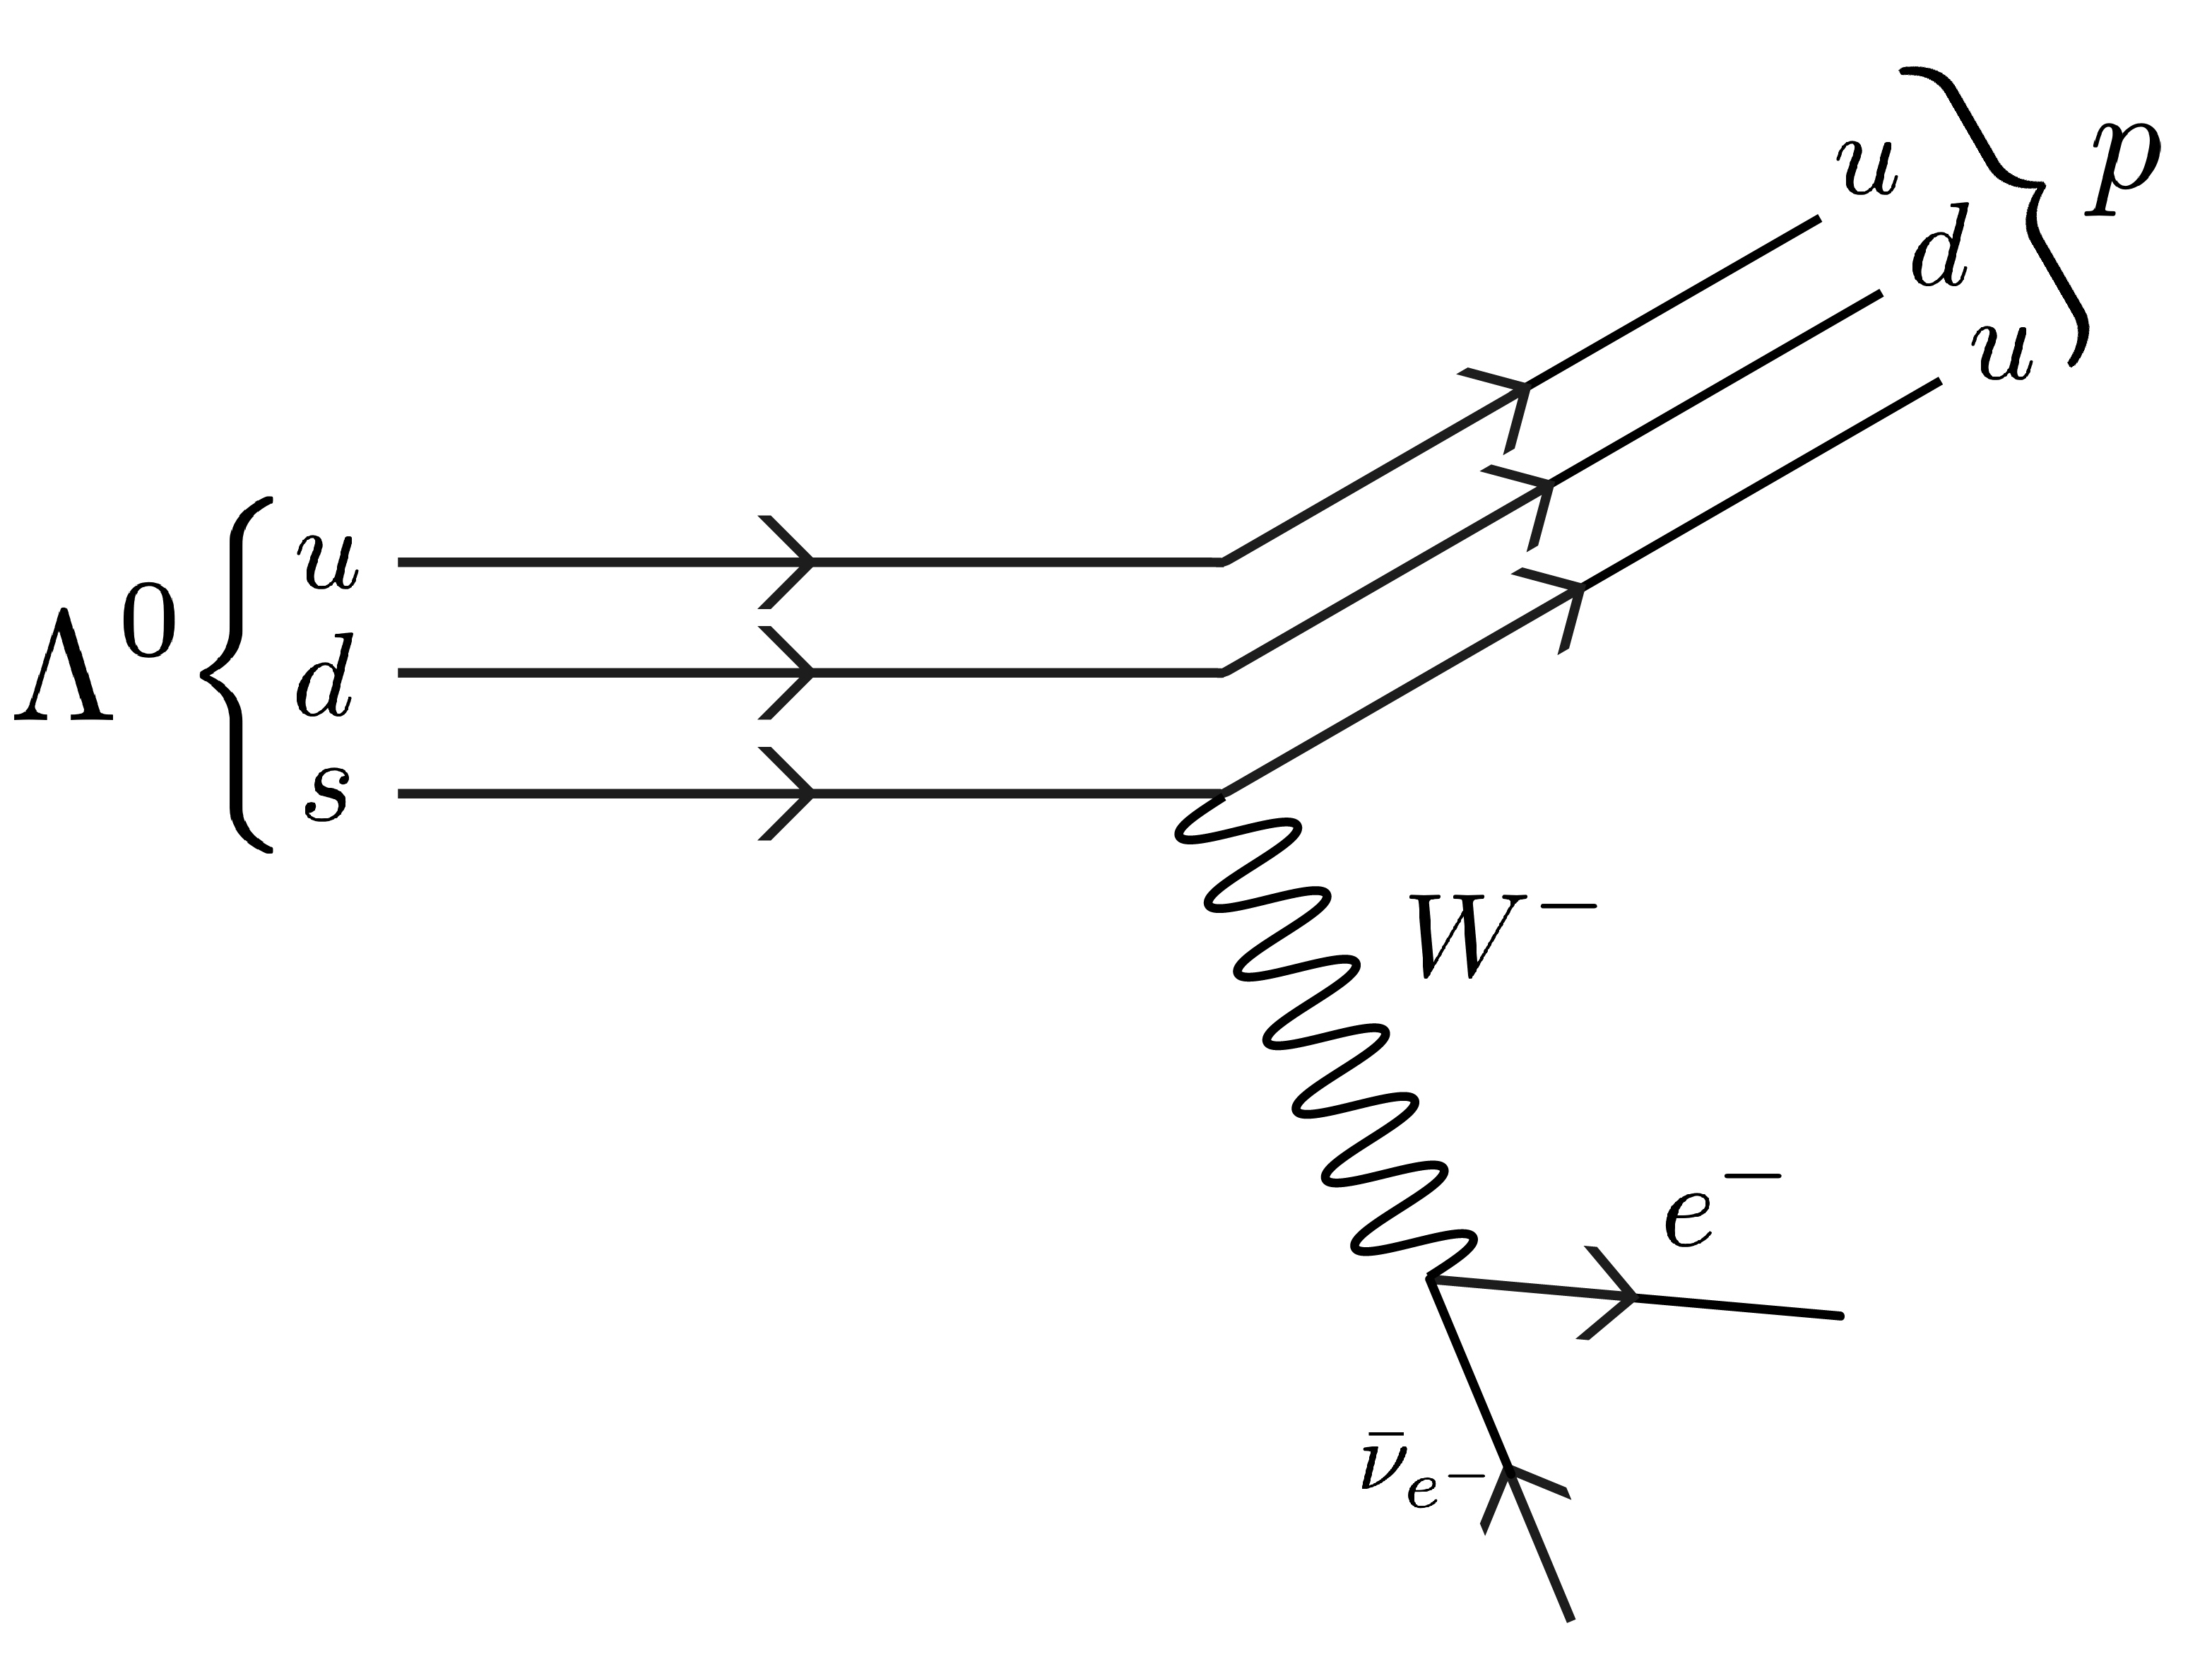
\includegraphics[scale=0.05]{Feynman/lambda0-01.jpg}
        \caption{$\Lambda^0 \to p + e^- + \Bar{\nu_e}$}
    \end{minipage}
    \hspace{0.1\textwidth}
    \begin{minipage}{0.4\textwidth}
        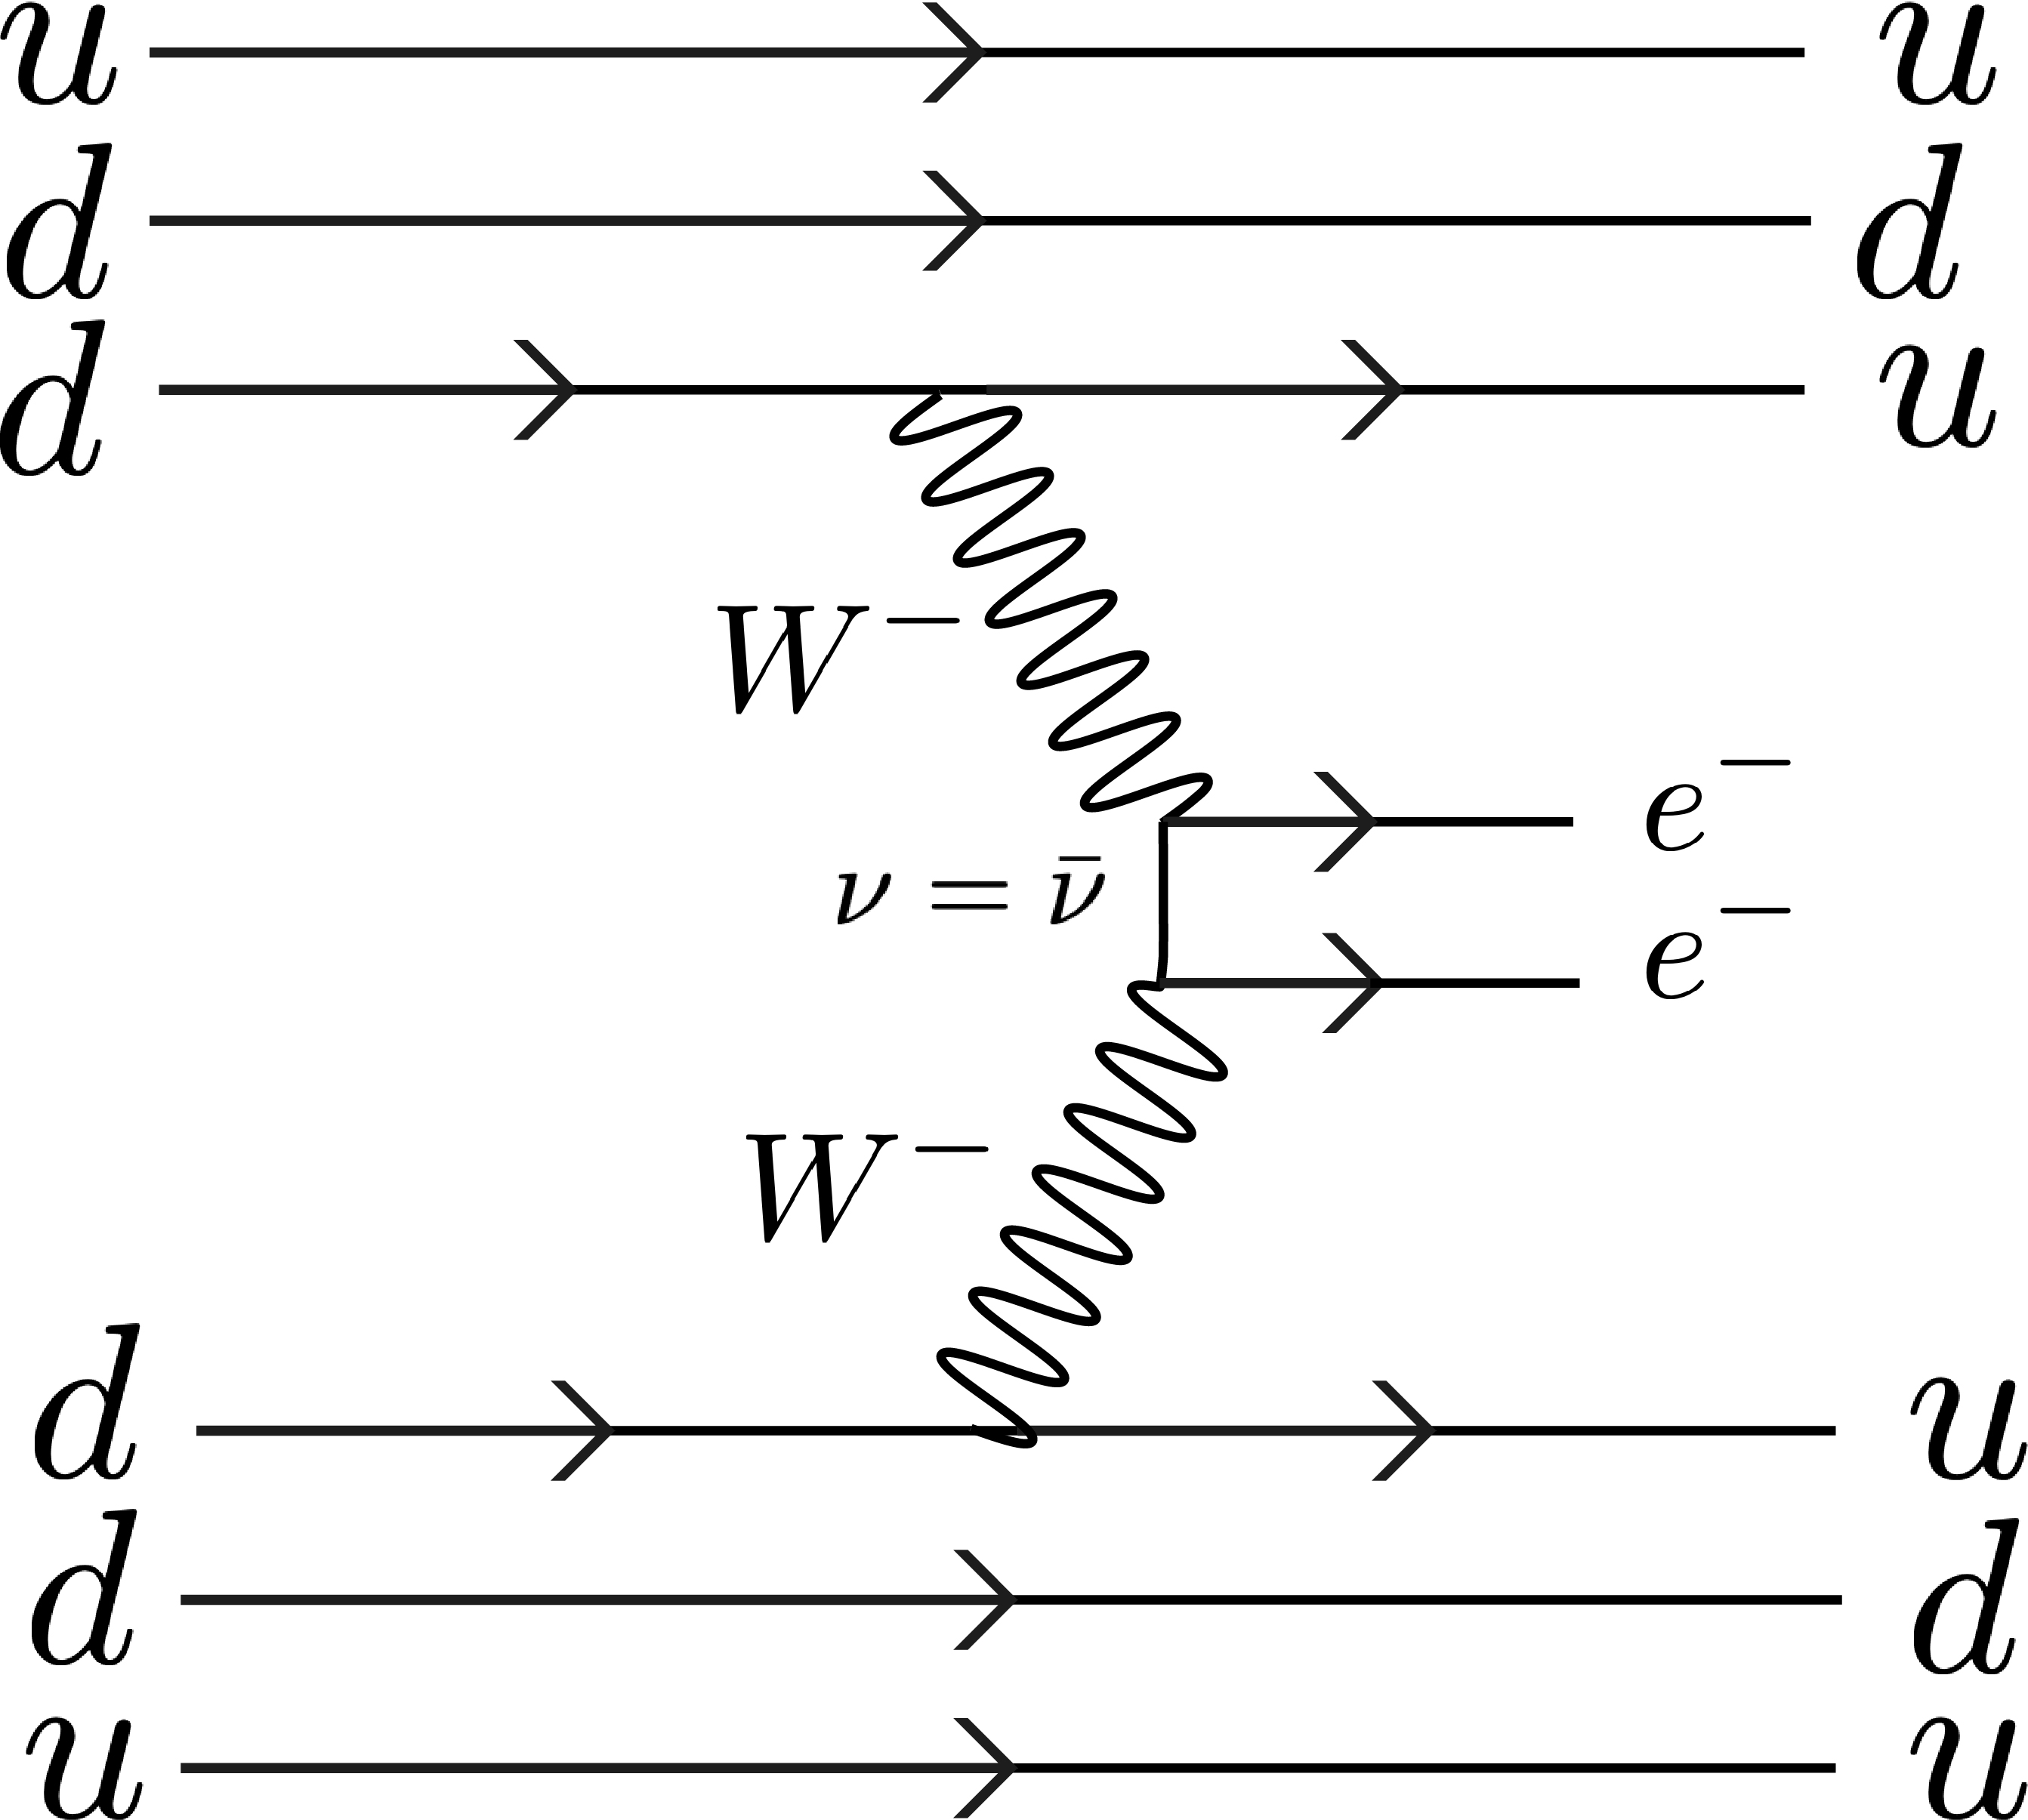
\includegraphics[scale=0.2]{Feynman/neutrinoless.jpg}
        \caption{$2n \to 2p + 2e^-$}
    \end{minipage}
    \vspace{30pt}
    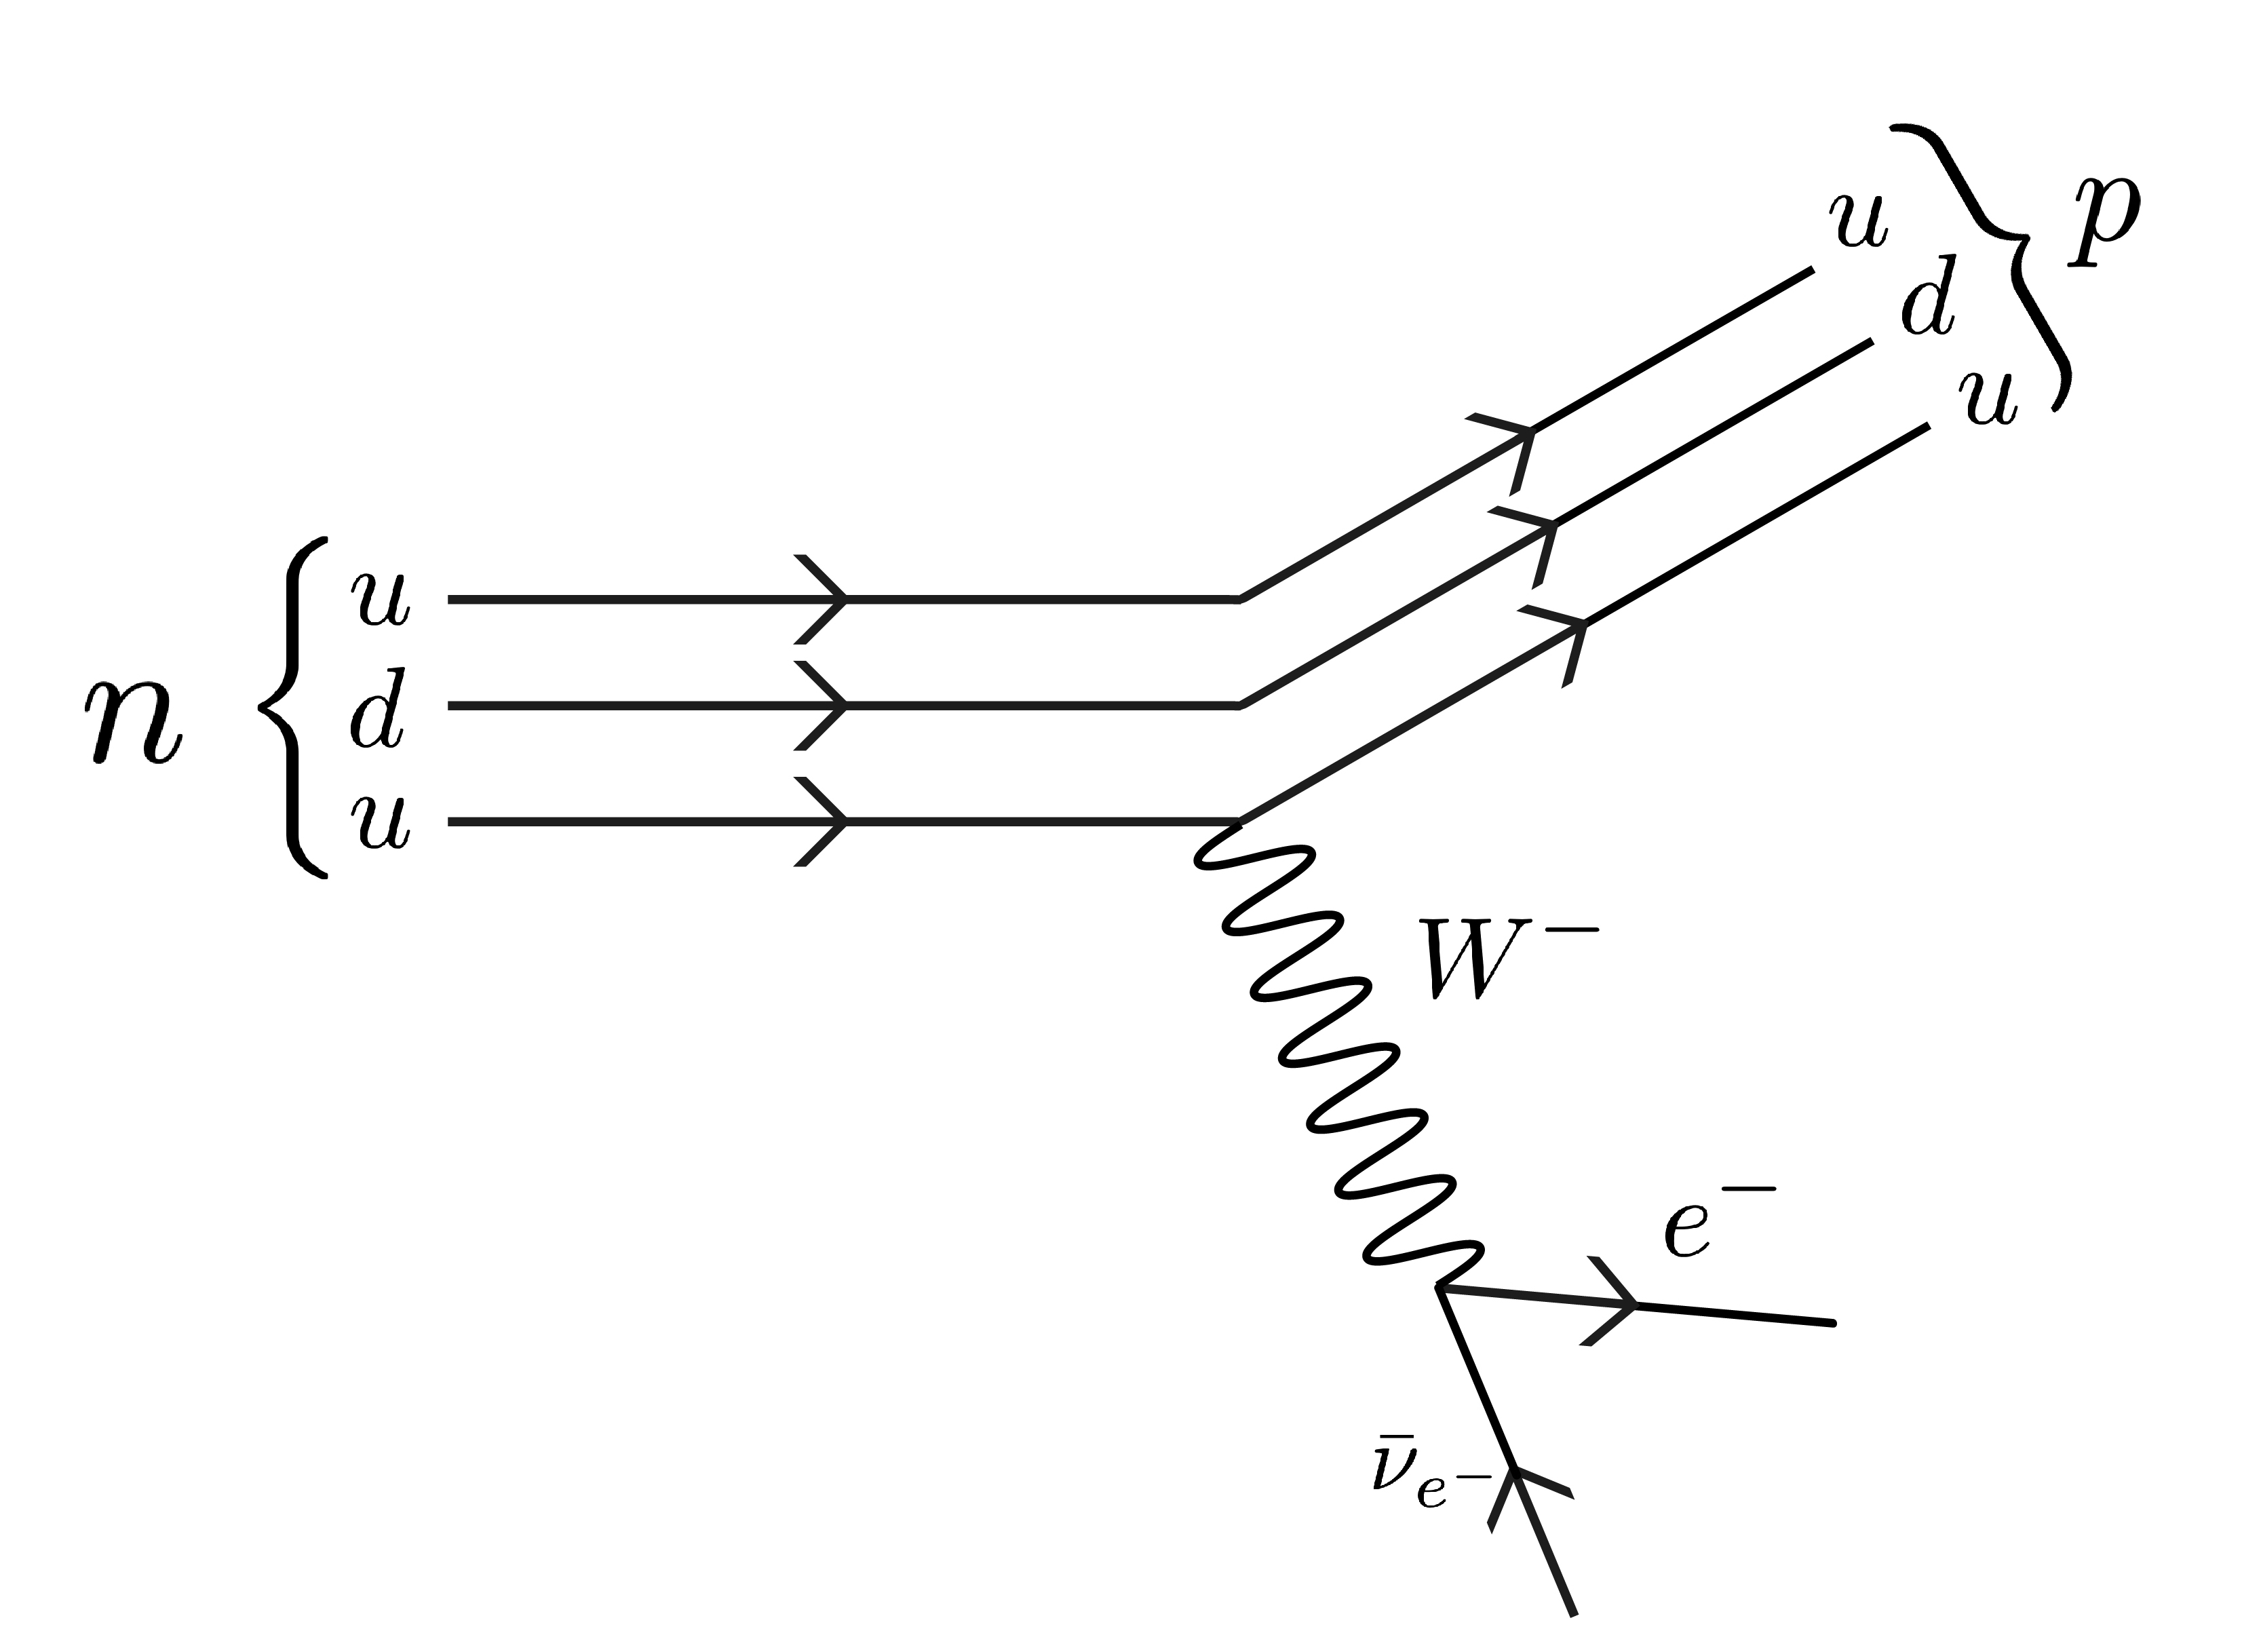
\includegraphics[scale=0.05]{Feynman/worldwouldbeboring-01.jpg}
    \caption{$2n \to 2p + 2e^- + 2\Bar{\nu_e}$}
    \label{fig:feynman_diagrams}
\end{figure}

\begin{table}[hbtp]
    \centering 
    \begin{tabular}{cccc}
        \toprule
            Process & Interaction & Typical Interaction time & Lifetime \\
        \midrule
            1 & electromagnetic & $10^{-14} \sim 10^{-20}$ & Not found\\
            3 & weak & $10^{-8} \sim 10^{-13}$ & $10^{-12}$ \\
            4 & weak & $10^{-8} \sim 10^{-13}$ & $10^{-10}$ \\
            5 & strong & $<10^{-22}$ & $10^{-24}$ \\
        \bottomrule
    \end{tabular}
\end{table}

Process 3 is not the most common decay for the bottom quark, hence extremely rare and suppressed. \\
Processes 7 and 8 differ by the presence of 2 antineutrinos. The process 8, namely the neutrinoless double beta decay,
is not allowed according to the Standard model because it violates the lepton number conservation. The observation of such 
decay would indeed confirm the Majorana nature of the neutrinos and the lepton number conservation rule would be violated. \\
When the neutron decays into 2 protons and 2 electrons without the neutrino, the energy is equally splitted to the generated particles 
according to their masses. On the opposite, when the antineutrinos are produced, part of the energy would be transferred to them,
but the portion is not fixed, hence it would produce a continuous energy spectrum.

